\documentclass[10pt]{article}
\usepackage[paperwidth=11in,paperheight=8.5in,margin=0in]{geometry}
\usepackage{tikz}
\usepackage[hidelinks]{hyperref}
\usepackage{graphicx}
\usepackage{array}
\usepackage{xcolor}
\usepackage{colortbl}

\definecolor{caninegray}{gray}{0.85}

\setlength{\parindent}{0pt}
\setlength{\parskip}{0pt}
\pagestyle{empty}

\setlength{\arrayrulewidth}{0.4pt}

\newcolumntype{L}[1]{>{\raggedright\arraybackslash}p{#1}}
\newcolumntype{C}[1]{>{\centering\arraybackslash}p{#1}}

\newcommand{\legendfont}{\fontsize{6.5}{8}\selectfont}
\newcommand{\smallfont}{\fontsize{7.5}{9}\selectfont}
\newcommand{\drnamefont}{\fontsize{9.75}{11.7}\selectfont}
\newcommand{\gridfont}{\fontsize{6}{7}\selectfont}
\newcommand{\titlefont}{\fontsize{20}{24}\selectfont}
\newcommand{\headerfont}{\fontsize{9.5}{11.4}\selectfont}

% Field-helper macros (all use black borders, no decoration overlay)
\newcommand{\inputf}[3]{\TextField[name=#1,width=#2,height=#3,bordercolor={0 0 0},borderwidth=0]{}}
\newcommand{\inputfm}[3]{\TextField[name=#1,multiline=true,width=#2,height=#3,bordercolor={0 0 0},borderwidth=0]{}}
\newcommand{\bcheck}[1]{\CheckBox[name=#1,width=0.10in,height=0.10in,bordercolor={0 0 0},borderwidth=0.5]{}}
% Grid cell: small TextField that fills a tooth-grid cell.
\newcommand{\gc}[1]{\TextField[name=#1,width=0.235in,height=0.14in,bordercolor={0 0 0},borderwidth=0]{}}
% Grid cell with gray background (used for canine C columns)
\newcommand{\gcc}[1]{\TextField[name=#1,width=0.235in,height=0.14in,bordercolor={0 0 0},borderwidth=0,backgroundcolor={0.85 0.85 0.85}]{}}

\begin{document}
\begin{Form}

%========================================================================
% PAGE 1
%========================================================================
\begin{tikzpicture}[remember picture, overlay,
    every node/.style={inner sep=0pt, outer sep=0pt}]

  % --- PATIENT STICKER BOX (top-left, decorative) ---------------------------
  \draw ([xshift=0.30in, yshift=-0.30in]current page.north west) rectangle
        ([xshift=2.90in, yshift=-2.05in]current page.north west);
  \node[anchor=north, font=\smallfont] at ([xshift=1.60in, yshift=-0.45in]current page.north west)
    {Patient Sticker};

  % --- PATIENT INFO BOX (Date / Doctor / Tech / Chief Complaint) -----------
  \node[anchor=north west] at ([xshift=3.65in, yshift=-0.30in]current page.north west) {%
    \smallfont
    \setlength{\tabcolsep}{4pt}%
    \begin{tabular}{|L{1.05in}|L{2.40in}|}
      \hline
      Date:            & \TextField[name=date,   width=2.40in, height=0.16in, bordercolor={0 0 0},borderwidth=0]{} \\ \hline
      Doctor:          & \TextField[name=doctor, width=2.40in, height=0.16in, bordercolor={0 0 0},borderwidth=0, value={Margaret Smith}]{} \\ \hline
      Tech:            & \TextField[name=tech,   width=2.40in, height=0.16in, bordercolor={0 0 0},borderwidth=0]{} \\ \hline
      Chief Complaint: & \TextField[name=chief,  multiline=true, width=2.40in, height=0.42in, bordercolor={0 0 0},borderwidth=0]{} \\ \hline
      \multicolumn{2}{|c|}{%
        \makebox[3.45in][c]{%
          Awake~\bcheck{awake}\hspace{0.35in}%
          Sedated~\bcheck{sedated}\hspace{0.35in}%
          Anesthetized~\bcheck{anesth}%
        }%
      } \\ \hline
    \end{tabular}};

  % --- VCA LOGO + TITLE (top-right) -----------------------------------------
  \node[anchor=north east] at ([xshift=-0.50in, yshift=-0.35in]current page.north east)
    {
\includegraphics[width=2.40in]{assets/logo_vca.png}};
  \node[anchor=north east, font=\titlefont] at ([xshift=-0.40in, yshift=-1.20in]current page.north east)
    {Canine Dental Chart};

  % --- TOOTH DIAGRAMS (left, extending to page bottom) ----------------------
  \node[anchor=north west] at ([xshift=0.30in, yshift=-2.50in]current page.north west)
    {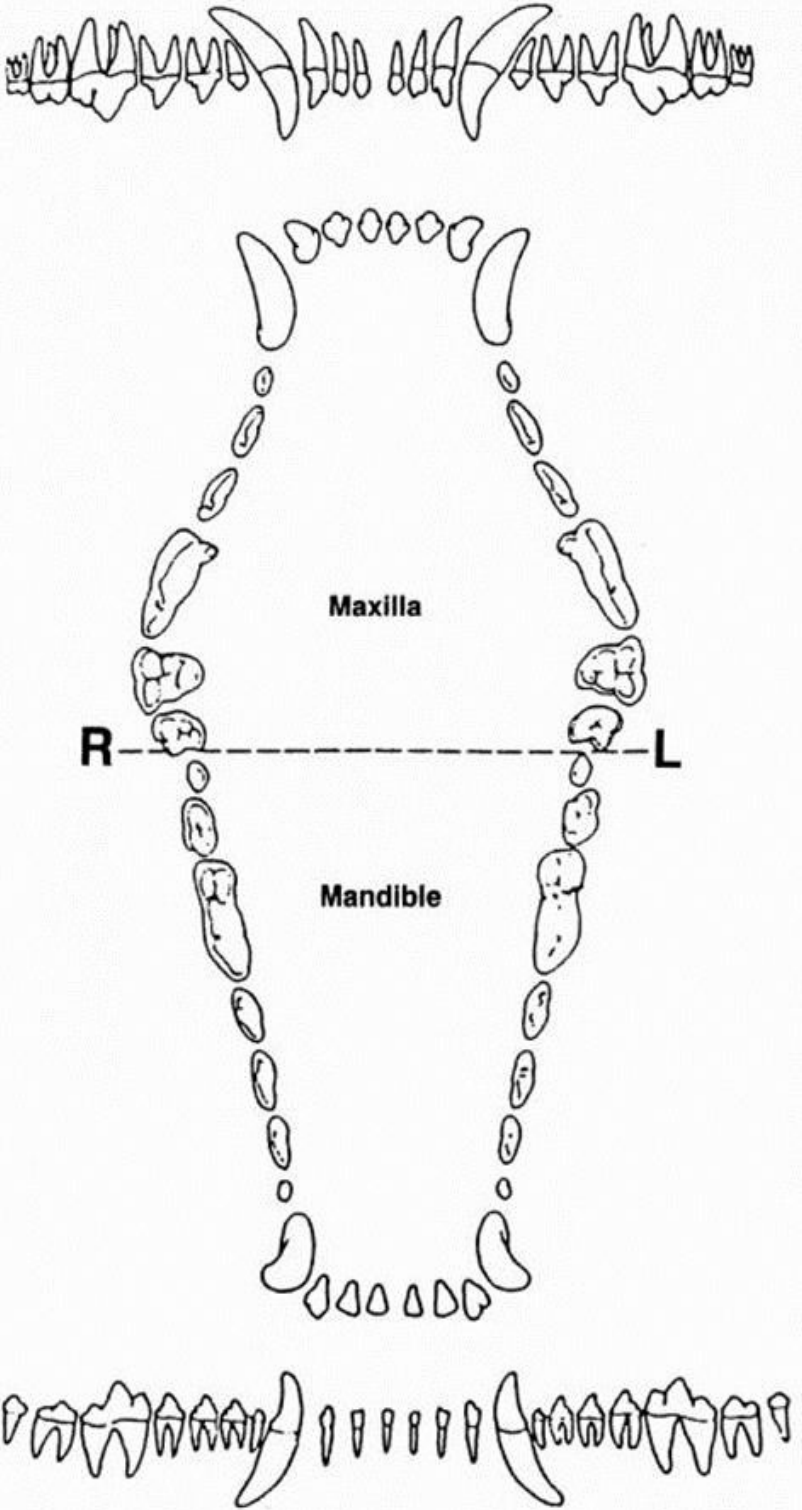
\includegraphics[height=4.73in]{assets/canine_diagrams_p2.png}};

  % --- ABBREVIATIONS LEGEND (right of diagrams) -----------------------------
  \node[anchor=north west] at ([xshift=3.65in, yshift=-1.70in]current page.north west) {%
    \legendfont
    \setlength{\tabcolsep}{2pt}
    \renewcommand{\arraystretch}{1.10}
    \begin{tabular}{@{}p{0.55in}p{1.85in}p{0.85in}p{1.85in}p{1.30in}@{}}
      MAL/1 & BV, DV, LABV, LV, MV, PV          & AT/AB           & Attrition/abrasion                       & N A -- Extraoral/facial \\
      MAL/2 & MAL/3 MAL/4                       & E/D, E/H        & Enamel/defection, hypoplasia             & \\
      CB/C,R & Crossbite caudal, rostral        & CA              & Caries                                   & \\
      T/SN, SR & Supernumerary tooth, root      & RTR             & Retained tooth root or reserve crown     & N A -- Lymph nodes \\
      DT    & Deciduous tooth                   & T/A, I, LUX     & Tooth/avulsed, impacted, luxated         & \\
      DT/P  & Persistent deciduous tooth        & T/NV            & Tooth/non-vital                          & \\
      PD0   & No perio dx (clinically normal)   & CL/B, L, P, T   & Chewing lesion                           & \\
      PD1   & Gingivitis (no bone loss)         & FB              & Foreign body                             & N A -- Buccal mucosa \\
      PD2   & Mild periodontitis (25\% attach loss)        & LAC/B, L, T   & Laceration/buccal, lip tongue & \\
      PD3   & Mod periodontitis (25--50\% attach loss)     & MN/FX MX/FX   & Jaw fractures                  & \\
      PD4   & Severe periodontitis ($>$50\% attach loss)   & SYM/S         & Symphyseal separation          & \\
      GE    & Gingival enlargement              & CFP, CFL        & Cleft palate, Cleft lip                  & N A -- Tongue \\
      GR    & Gingival recession                & ONF             & Oronasal fistula                         & \\
      ST, ST/CS & Stomatitis, caudal stomatitis & ESP             & Elongated soft palate                    & \\
      CU/ST/CS  & Contact mucosal ulcer/mucositis & TMJ/D, FX, LUX & TMJ dysplasia, fracture, luxation       & \\
      OM    & Oral mass                         & GH              & Gingival hyperplasia                     & N A -- Palate \\
      DTC   & Dentigerous cyst                  & PA/P            & Periapical pathology                     & \\
      T/FX  & Tooth fracture (EI, EF, UCF, CCF, UCRF, CCRF, RF) & T/DIL & Dilaceration                       & \\
      ABE   & Alveolar bone expansion           & T/FDR           & Fused roots                              & \\
      LN/E  & Lymph node enlargement            & T/U             & Tooth unerupted                          & N A -- Pharynx/Tonsils \\
      *SE   & Super eruption                    & *SI             & Intrinsic staining                       & \\
    \end{tabular}};

  % --- TOOTH GRID: MAXILLA (right of diagram, below abbreviations) ----------
  \node[anchor=north west] at ([xshift=3.65in, yshift=-4.40in]current page.north west) {%
    \fontsize{6.5}{8}\selectfont
    \setlength{\tabcolsep}{2pt}
    \renewcommand{\arraystretch}{1.55}
    \begin{tabular}{|>{\columncolor{caninegray}}L{0.50in}|*{6}{C{0.245in}|}>{\columncolor{caninegray}}C{0.245in}|*{6}{C{0.245in}|}>{\columncolor{caninegray}}C{0.245in}|*{6}{C{0.245in}|}}
      \hline
      \rowcolor{caninegray} Tooth        & M2  & M1  & P4  & P3  & P2  & P1  & C   & I3  & I2  & I1  & I1  & I2  & I3  & C   & P1  & P2  & P3  & P4  & M1  & M2  \\ \hline
      \rowcolor{caninegray} Triadan      & 110 & 109 & 108 & 107 & 106 & 105 & 104 & 103 & 102 & 101 & 201 & 202 & 203 & 204 & 205 & 206 & 207 & 208 & 209 & 210 \\ \hline
      Mobility     & \gc{g_110_mob} & \gc{g_109_mob} & \gc{g_108_mob} & \gc{g_107_mob} & \gc{g_106_mob} & \gc{g_105_mob} & \gcc{g_104_mob} & \gc{g_103_mob} & \gc{g_102_mob} & \gc{g_101_mob} & \gc{g_201_mob} & \gc{g_202_mob} & \gc{g_203_mob} & \gcc{g_204_mob} & \gc{g_205_mob} & \gc{g_206_mob} & \gc{g_207_mob} & \gc{g_208_mob} & \gc{g_209_mob} & \gc{g_210_mob} \\ \hline
      Recession    & \gc{g_110_rec} & \gc{g_109_rec} & \gc{g_108_rec} & \gc{g_107_rec} & \gc{g_106_rec} & \gc{g_105_rec} & \gcc{g_104_rec} & \gc{g_103_rec} & \gc{g_102_rec} & \gc{g_101_rec} & \gc{g_201_rec} & \gc{g_202_rec} & \gc{g_203_rec} & \gcc{g_204_rec} & \gc{g_205_rec} & \gc{g_206_rec} & \gc{g_207_rec} & \gc{g_208_rec} & \gc{g_209_rec} & \gc{g_210_rec} \\ \hline
      Pocket       & \gc{g_110_poc} & \gc{g_109_poc} & \gc{g_108_poc} & \gc{g_107_poc} & \gc{g_106_poc} & \gc{g_105_poc} & \gcc{g_104_poc} & \gc{g_103_poc} & \gc{g_102_poc} & \gc{g_101_poc} & \gc{g_201_poc} & \gc{g_202_poc} & \gc{g_203_poc} & \gcc{g_204_poc} & \gc{g_205_poc} & \gc{g_206_poc} & \gc{g_207_poc} & \gc{g_208_poc} & \gc{g_209_poc} & \gc{g_210_poc} \\ \hline
      Furcation    & \gc{g_110_fur} & \gc{g_109_fur} & \gc{g_108_fur} & \gc{g_107_fur} & \gc{g_106_fur} & \gc{g_105_fur} & \gcc{g_104_fur} & \gc{g_103_fur} & \gc{g_102_fur} & \gc{g_101_fur} & \gc{g_201_fur} & \gc{g_202_fur} & \gc{g_203_fur} & \gcc{g_204_fur} & \gc{g_205_fur} & \gc{g_206_fur} & \gc{g_207_fur} & \gc{g_208_fur} & \gc{g_209_fur} & \gc{g_210_fur} \\ \hline
      Hyperplasia  & \gc{g_110_hyp} & \gc{g_109_hyp} & \gc{g_108_hyp} & \gc{g_107_hyp} & \gc{g_106_hyp} & \gc{g_105_hyp} & \gcc{g_104_hyp} & \gc{g_103_hyp} & \gc{g_102_hyp} & \gc{g_101_hyp} & \gc{g_201_hyp} & \gc{g_202_hyp} & \gc{g_203_hyp} & \gcc{g_204_hyp} & \gc{g_205_hyp} & \gc{g_206_hyp} & \gc{g_207_hyp} & \gc{g_208_hyp} & \gc{g_209_hyp} & \gc{g_210_hyp} \\ \hline
      Calculus     & \gc{g_110_cal} & \gc{g_109_cal} & \gc{g_108_cal} & \gc{g_107_cal} & \gc{g_106_cal} & \gc{g_105_cal} & \gcc{g_104_cal} & \gc{g_103_cal} & \gc{g_102_cal} & \gc{g_101_cal} & \gc{g_201_cal} & \gc{g_202_cal} & \gc{g_203_cal} & \gcc{g_204_cal} & \gc{g_205_cal} & \gc{g_206_cal} & \gc{g_207_cal} & \gc{g_208_cal} & \gc{g_209_cal} & \gc{g_210_cal} \\ \hline
      Gingivitis   & \gc{g_110_gin} & \gc{g_109_gin} & \gc{g_108_gin} & \gc{g_107_gin} & \gc{g_106_gin} & \gc{g_105_gin} & \gcc{g_104_gin} & \gc{g_103_gin} & \gc{g_102_gin} & \gc{g_101_gin} & \gc{g_201_gin} & \gc{g_202_gin} & \gc{g_203_gin} & \gcc{g_204_gin} & \gc{g_205_gin} & \gc{g_206_gin} & \gc{g_207_gin} & \gc{g_208_gin} & \gc{g_209_gin} & \gc{g_210_gin} \\ \hline
      PD Stage     & \gc{g_110_pds} & \gc{g_109_pds} & \gc{g_108_pds} & \gc{g_107_pds} & \gc{g_106_pds} & \gc{g_105_pds} & \gcc{g_104_pds} & \gc{g_103_pds} & \gc{g_102_pds} & \gc{g_101_pds} & \gc{g_201_pds} & \gc{g_202_pds} & \gc{g_203_pds} & \gcc{g_204_pds} & \gc{g_205_pds} & \gc{g_206_pds} & \gc{g_207_pds} & \gc{g_208_pds} & \gc{g_209_pds} & \gc{g_210_pds} \\ \hline
    \end{tabular}};

  % --- TOOTH GRID: MANDIBLE (right of diagram, below maxilla) ---------------
  \node[anchor=north west] at ([xshift=3.65in, yshift=-6.55in]current page.north west) {%
    \fontsize{6.5}{8}\selectfont
    \setlength{\tabcolsep}{2pt}
    \renewcommand{\arraystretch}{1.55}
    \begin{tabular}{|>{\columncolor{caninegray}}L{0.50in}|*{7}{C{0.222in}|}>{\columncolor{caninegray}}C{0.222in}|*{6}{C{0.222in}|}>{\columncolor{caninegray}}C{0.222in}|*{7}{C{0.222in}|}}
      \hline
      \rowcolor{caninegray} Tooth        & M3  & M2  & M1  & P4  & P3  & P2  & P1  & C   & I3  & I2  & I1  & I1  & I2  & I3  & C   & P1  & P2  & P3  & P4  & M1  & M2  & M3  \\ \hline
      \rowcolor{caninegray} Triadan      & 411 & 410 & 409 & 408 & 407 & 406 & 405 & 404 & 403 & 402 & 401 & 301 & 302 & 303 & 304 & 305 & 306 & 307 & 308 & 309 & 310 & 311 \\ \hline
      Mobility     & \gc{g_411_mob} & \gc{g_410_mob} & \gc{g_409_mob} & \gc{g_408_mob} & \gc{g_407_mob} & \gc{g_406_mob} & \gc{g_405_mob} & \gcc{g_404_mob} & \gc{g_403_mob} & \gc{g_402_mob} & \gc{g_401_mob} & \gc{g_301_mob} & \gc{g_302_mob} & \gc{g_303_mob} & \gcc{g_304_mob} & \gc{g_305_mob} & \gc{g_306_mob} & \gc{g_307_mob} & \gc{g_308_mob} & \gc{g_309_mob} & \gc{g_310_mob} & \gc{g_311_mob} \\ \hline
      Recession    & \gc{g_411_rec} & \gc{g_410_rec} & \gc{g_409_rec} & \gc{g_408_rec} & \gc{g_407_rec} & \gc{g_406_rec} & \gc{g_405_rec} & \gcc{g_404_rec} & \gc{g_403_rec} & \gc{g_402_rec} & \gc{g_401_rec} & \gc{g_301_rec} & \gc{g_302_rec} & \gc{g_303_rec} & \gcc{g_304_rec} & \gc{g_305_rec} & \gc{g_306_rec} & \gc{g_307_rec} & \gc{g_308_rec} & \gc{g_309_rec} & \gc{g_310_rec} & \gc{g_311_rec} \\ \hline
      Pocket       & \gc{g_411_poc} & \gc{g_410_poc} & \gc{g_409_poc} & \gc{g_408_poc} & \gc{g_407_poc} & \gc{g_406_poc} & \gc{g_405_poc} & \gcc{g_404_poc} & \gc{g_403_poc} & \gc{g_402_poc} & \gc{g_401_poc} & \gc{g_301_poc} & \gc{g_302_poc} & \gc{g_303_poc} & \gcc{g_304_poc} & \gc{g_305_poc} & \gc{g_306_poc} & \gc{g_307_poc} & \gc{g_308_poc} & \gc{g_309_poc} & \gc{g_310_poc} & \gc{g_311_poc} \\ \hline
      Furcation    & \gc{g_411_fur} & \gc{g_410_fur} & \gc{g_409_fur} & \gc{g_408_fur} & \gc{g_407_fur} & \gc{g_406_fur} & \gc{g_405_fur} & \gcc{g_404_fur} & \gc{g_403_fur} & \gc{g_402_fur} & \gc{g_401_fur} & \gc{g_301_fur} & \gc{g_302_fur} & \gc{g_303_fur} & \gcc{g_304_fur} & \gc{g_305_fur} & \gc{g_306_fur} & \gc{g_307_fur} & \gc{g_308_fur} & \gc{g_309_fur} & \gc{g_310_fur} & \gc{g_311_fur} \\ \hline
      Hyperplasia  & \gc{g_411_hyp} & \gc{g_410_hyp} & \gc{g_409_hyp} & \gc{g_408_hyp} & \gc{g_407_hyp} & \gc{g_406_hyp} & \gc{g_405_hyp} & \gcc{g_404_hyp} & \gc{g_403_hyp} & \gc{g_402_hyp} & \gc{g_401_hyp} & \gc{g_301_hyp} & \gc{g_302_hyp} & \gc{g_303_hyp} & \gcc{g_304_hyp} & \gc{g_305_hyp} & \gc{g_306_hyp} & \gc{g_307_hyp} & \gc{g_308_hyp} & \gc{g_309_hyp} & \gc{g_310_hyp} & \gc{g_311_hyp} \\ \hline
      Calculus     & \gc{g_411_cal} & \gc{g_410_cal} & \gc{g_409_cal} & \gc{g_408_cal} & \gc{g_407_cal} & \gc{g_406_cal} & \gc{g_405_cal} & \gcc{g_404_cal} & \gc{g_403_cal} & \gc{g_402_cal} & \gc{g_401_cal} & \gc{g_301_cal} & \gc{g_302_cal} & \gc{g_303_cal} & \gcc{g_304_cal} & \gc{g_305_cal} & \gc{g_306_cal} & \gc{g_307_cal} & \gc{g_308_cal} & \gc{g_309_cal} & \gc{g_310_cal} & \gc{g_311_cal} \\ \hline
      Gingivitis   & \gc{g_411_gin} & \gc{g_410_gin} & \gc{g_409_gin} & \gc{g_408_gin} & \gc{g_407_gin} & \gc{g_406_gin} & \gc{g_405_gin} & \gcc{g_404_gin} & \gc{g_403_gin} & \gc{g_402_gin} & \gc{g_401_gin} & \gc{g_301_gin} & \gc{g_302_gin} & \gc{g_303_gin} & \gcc{g_304_gin} & \gc{g_305_gin} & \gc{g_306_gin} & \gc{g_307_gin} & \gc{g_308_gin} & \gc{g_309_gin} & \gc{g_310_gin} & \gc{g_311_gin} \\ \hline
      PD Stage     & \gc{g_411_pds} & \gc{g_410_pds} & \gc{g_409_pds} & \gc{g_408_pds} & \gc{g_407_pds} & \gc{g_406_pds} & \gc{g_405_pds} & \gcc{g_404_pds} & \gc{g_403_pds} & \gc{g_402_pds} & \gc{g_401_pds} & \gc{g_301_pds} & \gc{g_302_pds} & \gc{g_303_pds} & \gcc{g_304_pds} & \gc{g_305_pds} & \gc{g_306_pds} & \gc{g_307_pds} & \gc{g_308_pds} & \gc{g_309_pds} & \gc{g_310_pds} & \gc{g_311_pds} \\ \hline
    \end{tabular}};

  % --- FOOTER -------------------------------------------------------
  \node[anchor=south east, font=\smallfont] at ([xshift=-0.30in, yshift=0.20in]current page.south east)
    {1 of 2};

\end{tikzpicture}

\newpage

%========================================================================
% PAGE 2
%========================================================================
\begin{tikzpicture}[remember picture, overlay,
    every node/.style={inner sep=0pt, outer sep=0pt}]

  % --- NERVE BLOCK TABLE (top-left) -----------------------------------------
  \node[anchor=north west] at ([xshift=0.30in, yshift=-0.30in]current page.north west) {%
    \smallfont
    \setlength{\tabcolsep}{3pt}
    \renewcommand{\arraystretch}{1.15}
    \begin{tabular}{|L{1.55in}|C{0.55in}|C{0.55in}|}
      \hline
      \textbf{Nerve Block 0.5\% Ropivacaine} & \textbf{RIGHT} & \textbf{LEFT} \\ \hline
      Infraorbital      & \TextField[name=nb_io_r,  width=0.30in, height=0.16in, bordercolor={0 0 0},borderwidth=0]{}~mL & \TextField[name=nb_io_l,  width=0.30in, height=0.16in, bordercolor={0 0 0},borderwidth=0]{}~mL \\ \hline
      Inferior Alveolar & \TextField[name=nb_ia_r,  width=0.30in, height=0.16in, bordercolor={0 0 0},borderwidth=0]{}~mL & \TextField[name=nb_ia_l,  width=0.30in, height=0.16in, bordercolor={0 0 0},borderwidth=0]{}~mL \\ \hline
      Mental            & \TextField[name=nb_men_r, width=0.30in, height=0.16in, bordercolor={0 0 0},borderwidth=0]{}~mL & \TextField[name=nb_men_l, width=0.30in, height=0.16in, bordercolor={0 0 0},borderwidth=0]{}~mL \\ \hline
      Other             & \TextField[name=nb_oth_r, width=0.50in, height=0.16in, bordercolor={0 0 0},borderwidth=0]{}    & \TextField[name=nb_oth_l, width=0.50in, height=0.16in, bordercolor={0 0 0},borderwidth=0]{}    \\ \hline
    \end{tabular}};

  % --- TOOTH DIAGRAMS (left middle) -----------------------------------------
  \node[anchor=north west] at ([xshift=0.55in, yshift=-1.85in]current page.north west)
    {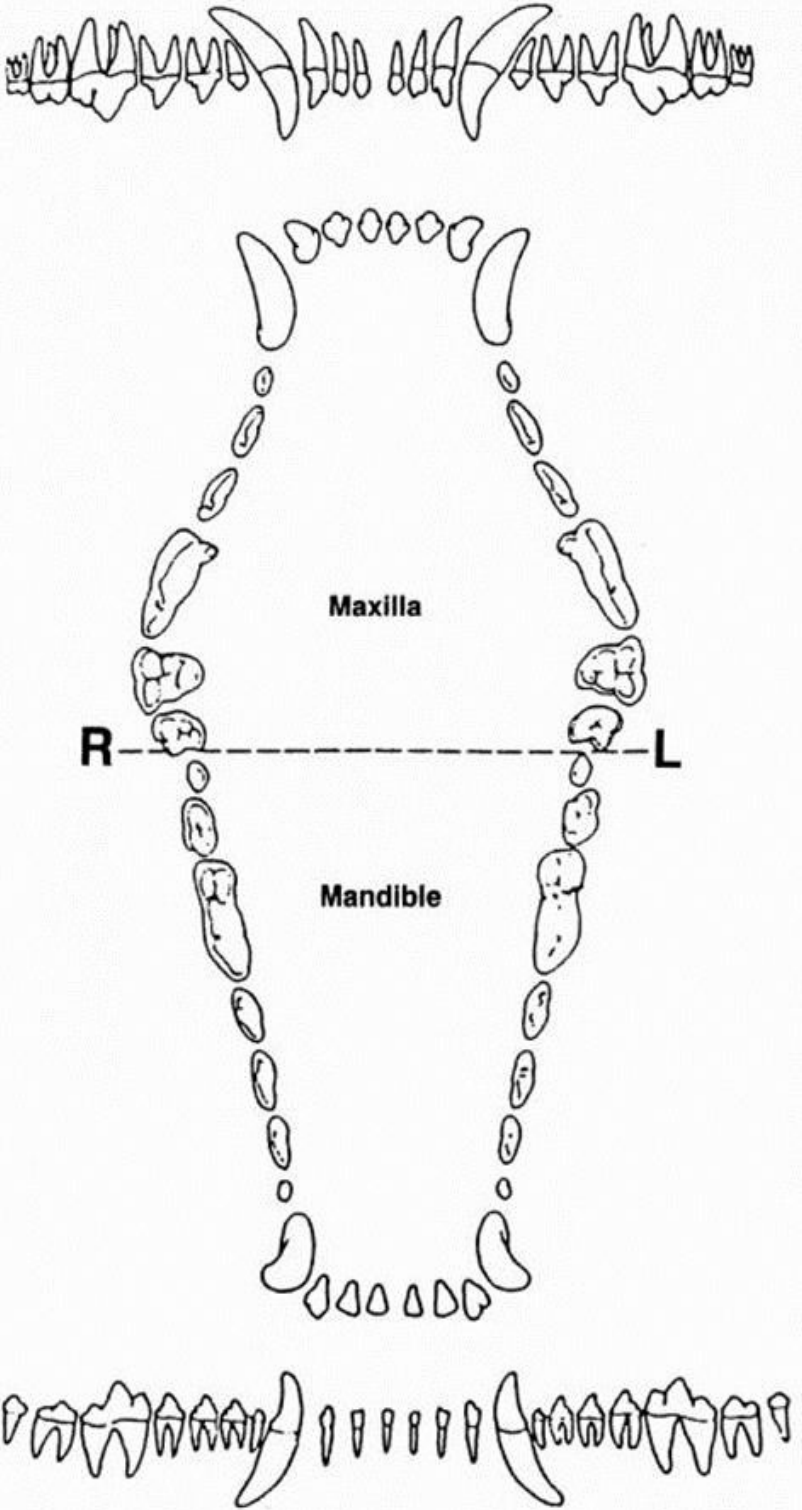
\includegraphics[height=4.20in]{assets/canine_diagrams_p2.png}};

  % --- ABBREVIATIONS LEGEND (single tall column) ----------------------------
  \node[anchor=north west] at ([xshift=3.30in, yshift=-0.30in]current page.north west) {%
    \legendfont
    \setlength{\tabcolsep}{2pt}
    \renewcommand{\arraystretch}{1.05}
    \begin{tabular}{@{}p{0.85in}p{2.30in}@{}}
      RAD             & Rads (Dental, CDR, CT Scan, Plain Film) \\
      B/I B/E         & Biopsy-incisional/excisional \\
      CS              & Culture/Sensitivity \\
      PRO             & Professional prophylaxis \\
      GC              & Gingival curettage \\
      RP/C            & Closed root planing \\
      RP/O            & Open root planing \\
      GV              & Gingivoplasty/gingivectomy \\
      F/AP            & Apically repositioned flap \\
      F/CO            & Coronally repositioned flap \\
      F/LA            & Laterally positioned flap \\
      CR/L            & Crown lengthening (Type 1, 2, 3) \\
      GF/B            & Bone graft \\
      GTR             & Guided tissue regeneration \\
      GF/G            & Gingival graft \\
      SPL/AC, C, W/R  & Splint acrylic, composite, wire reinforced \\
      RCT             & Standard root canal therapy \\
      RCT/S           & Surgical root canal therapy \\
      TRX             & Tooth partial resection (hemisection) \\
      CR/A            & Crown amputation \\
      CR/XP           & Crown reduction \\
      VPT             & Vital pulp therapy \\
      PCD, PCI        & Direct/indirect pulp capping \\
      CRA             & Crown amputation \\
      APN             & Apexification \\
      APG             & Apexogenesis \\
      R, R/C, I, A    & Restoration, composite, GI, amalgam \\
      IMP             & Implant \\
      F               & Flap \\
      X               & Extr.-closed no sectioning \\
      XS              & Extr.-closed, w/ sectioning \\
      XSS             & Extr.-open \\
      ALV             & Alveolectomy/alveoloplasty \\
      ONF/R           & Oronasal fistula repair \\
      CFP/R           & Cleft palate repair \\
      CFL/R           & Cleft lip repair \\
      S/P             & Palate surgery \\
      S/M             & Mandibulectomy (partial) \\
      S/X             & Maxillectomy (partial) \\
      FRE             & Frenoplasty \\
      SYM/R           & Symphyseal repair \\
      FX/R            & Jaw fracture repair (j. fx. rp.) \\
      FX/R/PL         & Plate j. fx. rp. \\
      FX/R/S          & Screw j. fx. rp. \\
      FX/R/WIR        & Wire j. fx. rp. \\
      FX/R/WIR/C      & Cerclage wire j. fx. rp. \\
      FX/R/WIR/ID     & Interdental wire j. fx. rp. \\
      FX/R/WIRE/OS    & Osseous wire j. fx. rp. \\
      FX/R/WIR/IDS    & Splinting \\
      FX/R/MMF        & Maxillary mandibular fixation \\
      CON/X           & Condylectomy \\
      LUX/R           & Reduction of TMJ luxation \\
      CBU             & Core build up \\
      CR/P            & Crown preparation \\
      CR/M            & Crown metal \\
      CR/PFM          & Crown porcelain fused to metal \\
      IMF             & Impressions full mouth \\
      IP/AC, C, M     & Inclined plane/acrylic, composite, metal \\
      OA/I            & Ortho appliance -- install \\
      OA/A            & Ortho appliance -- adjust \\
      OA/R            & Ortho appliance -- remove \\
      OA/BKT, BU      & Ortho app./bracket, button \\
      OA/EC, WIR      & Ortho app./elastic, wire \\
    \end{tabular}};

  % --- TREATMENT AND SURGERY REPORT (top right input box) -------------------
  \node[anchor=north west, font=\headerfont] at ([xshift=6.70in, yshift=-0.30in]current page.north west)
    {\textbf{Treatment and Surgery Report:}};
  \node[anchor=north west] at ([xshift=6.70in, yshift=-0.50in]current page.north west) {%
    \TextField[name=treatment_report, multiline=true,
               width=4.00in, height=2.30in,
               borderwidth=0, bordercolor={0 0 0},
               value=]{}};

  % --- INSTRUCTIONS & MEDICATIONS (middle right input box) ------------------
  \node[anchor=north west, font=\headerfont] at ([xshift=6.70in, yshift=-2.95in]current page.north west)
    {\textbf{Instructions \& Medications:}};
  \node[anchor=north west] at ([xshift=6.70in, yshift=-3.15in]current page.north west) {%
    \TextField[name=instructions_meds, multiline=true,
               width=4.00in, height=2.20in,
               borderwidth=0, bordercolor={0 0 0},
               value=]{}};

  % --- FOLLOW-UP (bottom right input box) -----------------------------------
  \node[anchor=north west, font=\headerfont] at ([xshift=6.70in, yshift=-5.50in]current page.north west)
    {\textbf{Follow-up:}};
  \node[anchor=north west] at ([xshift=6.70in, yshift=-5.70in]current page.north west) {%
    \TextField[name=followup, multiline=true,
               width=4.00in, height=2.25in,
               borderwidth=0, bordercolor={0 0 0},
               value=]{}};

  % --- FOOTER -------------------------------------------------------
  \node[anchor=south east, font=\smallfont] at ([xshift=-0.30in, yshift=0.20in]current page.south east)
    {2 of 2};

\end{tikzpicture}

\end{Form}
\end{document}
